\section{Experimental Evaluation}
\label{sec:results}

\begin{figure*}[ht]
  \centering
  \begin{subfigure}[b]{.45\textwidth}
    \subcaptionbox*{}{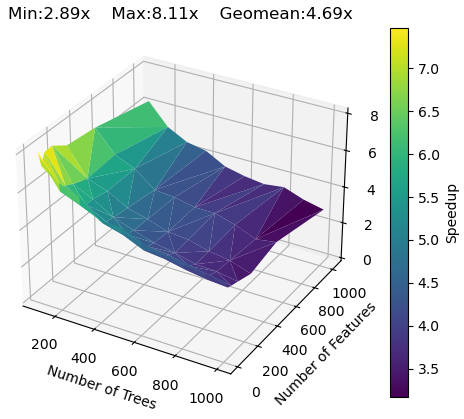
\includegraphics[width=\textwidth]{figures/RandomModels/kernel_speedup_b512_depth8.png}}
    \caption{Batch size 512, depth 8}
  \end{subfigure}
  \begin{subfigure}[b]{.45\textwidth}
    \subcaptionbox*{}{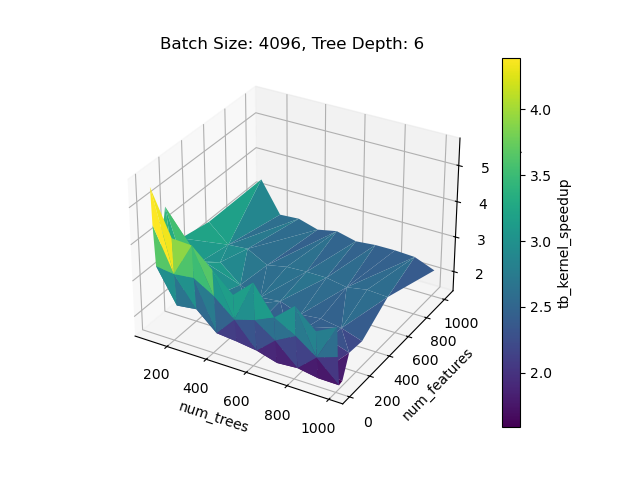
\includegraphics[width=\textwidth]{figures/RandomModels/kernel_speedup_b4096_depth6.png}}
    \caption{Batch size 4096, depth 6}
  \end{subfigure}
  \hfill
  \caption{\Treebeard{} vs RAPIDs Kernel Time Speedup on NVIDIA RTX 4060 for several randomly generated models.}
\end{figure*}

\begin{figure}[htb]
  \centering
  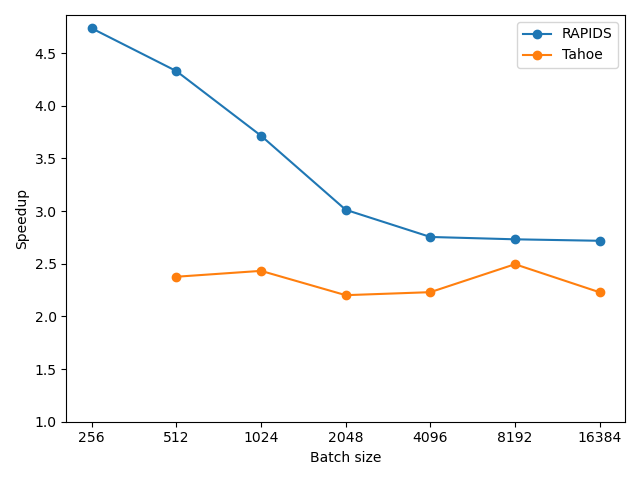
\includegraphics[width=0.75\linewidth]{figures/geomean_speedup_4060_kernel_time.png}
  \caption{\Treebeard{} vs RAPIDs and Tahoe Kernel Time Speedup on NVIDIA RTX 4060}
  \label{Fig:TBvsRAPIDsTahoe_4060_Speedup}
\end{figure}

\begin{figure}[htb]
  \centering
  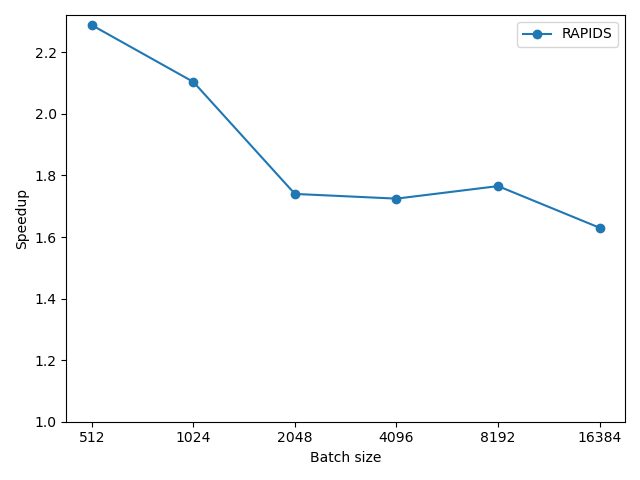
\includegraphics[width=0.75\linewidth]{figures/geomean_speedup_4060_total_time.png}
  \caption{\Treebeard{} vs RAPIDs Total Time Speedup on NVIDIA RTX 4060.}
  \label{Fig:TBvsRAPIDs_4060_TotalTimeSpeedup}
\end{figure}

\begin{figure*}[ht]
  \centering
  \begin{subfigure}[b]{.45\textwidth}
    \subcaptionbox*{}{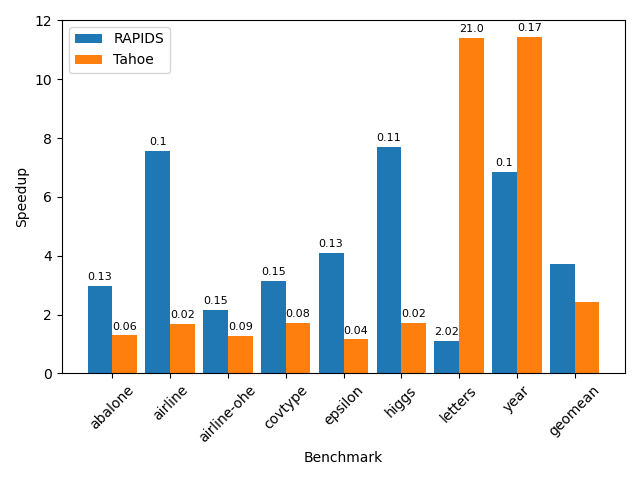
\includegraphics[width=\textwidth]{figures/speedup_bar_graph_1024.png}}
    \caption{Batch size 1024}
  \end{subfigure}
  \begin{subfigure}[b]{.45\textwidth}
    \subcaptionbox*{}{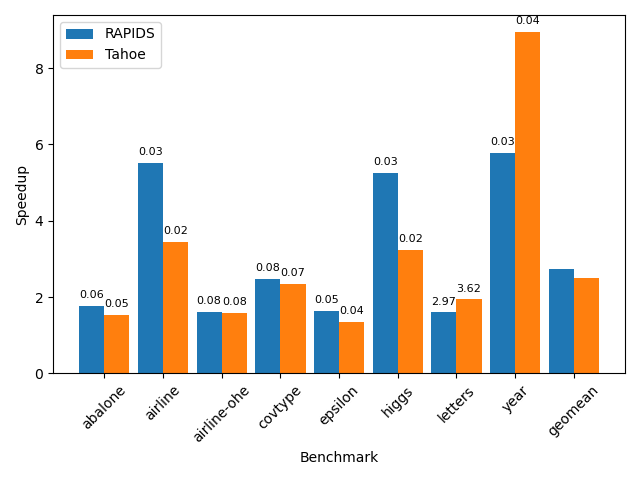
\includegraphics[width=\textwidth]{figures/speedup_bar_graph_8192.png}}
    \caption{Batch size 8192}
  \end{subfigure}
  \hfill
  \caption{Kernel time speedup of \Treebeard{} vs RAPIDs on NVIDIA RTX 4060. Numbers on the bars are 
  inference times per sample in $\mu$s for RAPIDs and Tahoe.}
\end{figure*}

\begin{figure}[htb]
  \centering
  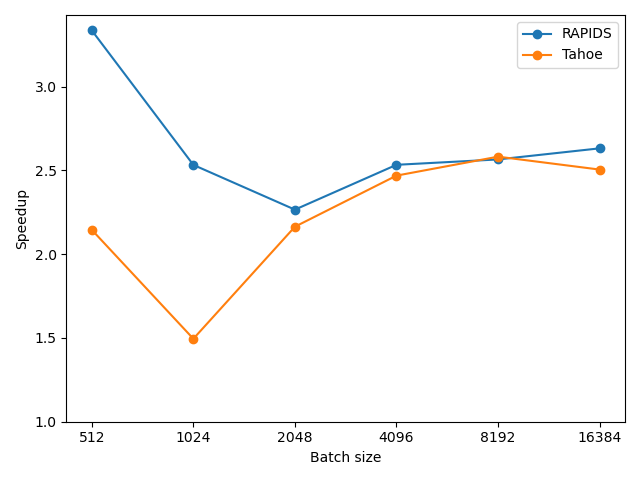
\includegraphics[width=0.75\linewidth]{figures/geomean_speedup_T400_kernel_time.png}
  \caption{\Treebeard{} vs RAPIDs and Tahoe Kernel Time Speedup on NVIDIA T400.}
  \label{Fig:TBvsRAPIDsTahoe_T400_Speedup}
\end{figure}

\begin{figure*}[ht]
  \centering
  \begin{subfigure}[b]{.45\textwidth}
    \subcaptionbox*{}{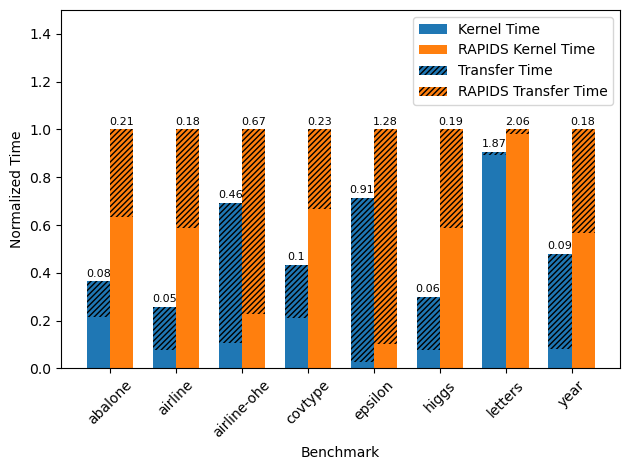
\includegraphics[width=\textwidth]{figures/abs_times_bar_graph_1024.png}}
    \caption{Batch size 1024.}
  \end{subfigure}
  \begin{subfigure}[b]{.45\textwidth}
    \subcaptionbox*{}{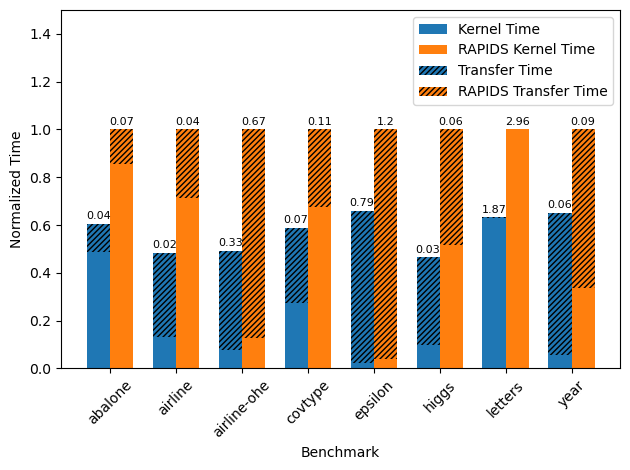
\includegraphics[width=\textwidth]{figures/abs_times_bar_graph_8192.png}}
    \caption{Batch size 8192.}
  \end{subfigure}
  \hfill
  \caption{\Treebeard{} vs RAPIDs total time comparison on NVIDIA RTX 4060. Numbers on the bars are the times 
  per sample in $\mu$s for \Treebeard{} and RAPIDs. Times for each benchmark are normalized w.r.t the RAPIDs time for that benchmark.}
\end{figure*}

\begin{figure}[htb]
  \centering
  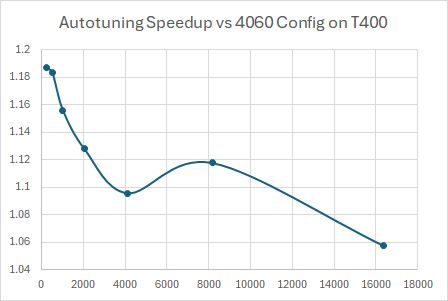
\includegraphics[width=0.75\linewidth]{figures/AutotuningSpeedupvs4060Sched_T400.png}
  \caption{Autotuning heuristics speedup vs best 4060 schedule on T400.}
  \label{Fig:AutotuningSpeedupvs4060Sched_T400}
\end{figure}

\begin{figure}[htb]
  \centering
  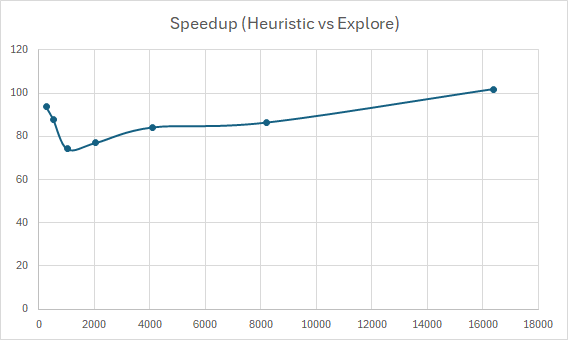
\includegraphics[width=0.75\linewidth]{figures/HeuristicVsFullExplore_Speedup.png}
  \caption{Autotuning heuristic compile time speedup vs full schedule exploration.}
  \label{Fig:HeuristicVsFullExplore_Speedup}
\end{figure}

\begin{figure}[htb]
  \centering
  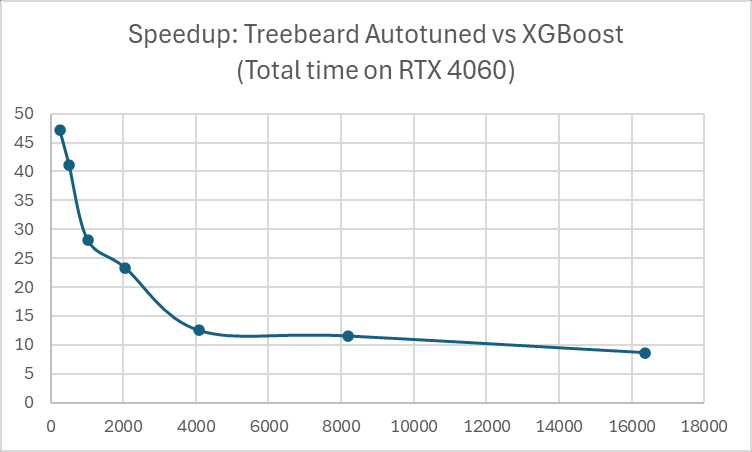
\includegraphics[width=0.75\linewidth]{figures/TBvsXGB_TotalTime.png}
  \caption{\Treebeard{} vs XGBoost Speedup on RTX 4060.}
  \label{Fig:TBvsXGBoost_Speedup}
\end{figure}

\begin{figure}[htb]
  \centering
  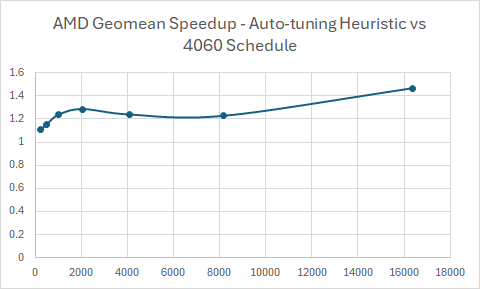
\includegraphics[width=0.75\linewidth]{figures/AMD_MI210_ATHeuristicVs4060Sched_speedup.png}
  \caption{Autotuning heuristics speedup vs best 4060 schedule on MI210.}
  \label{Fig:AMD_MI210_ATHeuristicVs4060Sched_speedup}
\end{figure}

